\documentclass[11pt, oneside]{article}   	% use "amsart" instead of "article" for AMSLaTeX format
\usepackage{geometry}                		% See geometry.pdf to learn the layout options. There are lots.
\geometry{letterpaper}                   		% ... or a4paper or a5paper or ... 
%\geometry{landscape}                		% Activate for for rotated page geometry
%\usepackage[parfill]{parskip}    		% Activate to begin paragraphs with an empty line rather than an indent
\usepackage{graphicx}				% Use pdf, png, jpg, or eps� with pdflatex; use eps in DVI mode
								% TeX will automatically convert eps --> pdf in pdflatex		
\usepackage{amssymb}
\usepackage{amsmath}

\title{All 6 trig functions}
%\author{The Author}
\date{}							% Activate to display a given date or no date

\graphicspath{{/Users/telliott_admin/Dropbox/Tex/png/}}

\begin{document}

\maketitle
%\section{}
% \subsection*{R code}
% \begin{lstlisting}  \end{lstlisting}
% \begin{center} 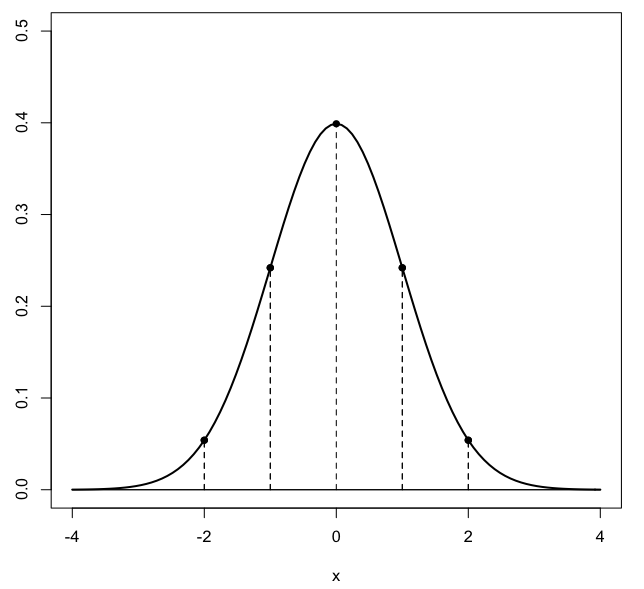
\includegraphics [scale=0.6] {gauss3.png} \end{center}
% \begin{bmatrix} a  &  b \\ c  &  d \end{bmatrix}
% \bigg |_

\large
\begin{center} 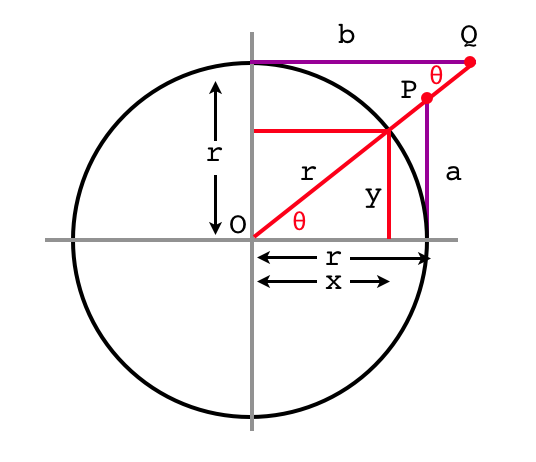
\includegraphics [scale=0.5] {sixfuncs1.png} \end{center}
Consider a unit circle with radius $r=1$ and $y/r = sin\ \theta$ and $x/r = cos\ \theta$.  Extend the radius with the angle $\theta$ and then draw the vertical connector $a$ and horizontal connector $b$.  The original triangle with sides $x,y,r$ is similar to the triangle with sides $r,a,OP$, and both are similar to the triangle with sides $b,r,OQ$.
\[ x,y,r \sim r,a,OP, \sim b,r,OQ \]
By similar $\triangle$
\[ a/r = y/x = tan \ \theta \]
But $r=1$ so 
\[ a = tan \ \theta \]
If you imagine a point moving around the circle $a$ will get very large as $\theta \to \pi/2$, and in fact, becomes $\infty$ there.
\vspace {2 mm}

\noindent The segment $OP$ is (by similar $\triangle$) to $a$ as
\[ OP/a = r/y = 1/y = 1/cos\ \theta = sec\ \theta \]

The horizontal from the y-axis to Q is $b$.  Consider $\theta$ near the top of the figure.  By similar $\triangle$, the relations we had were
\[ x,y,r \sim r,a,OP, \sim b,r,OQ \]
\[ r/b = y/x = tan \ \theta  \]
since $r = 1$
\[ b = r/tan \ \theta = 1/tan \ \theta = cot \ \theta \]
%\[ b/OQ = cos\  \theta \]
Finally
\[ r/OQ = 1/OQ = sin \ \theta \]
\[ OQ = 1/sin \ \theta = csc\ \theta \]

\begin{center} 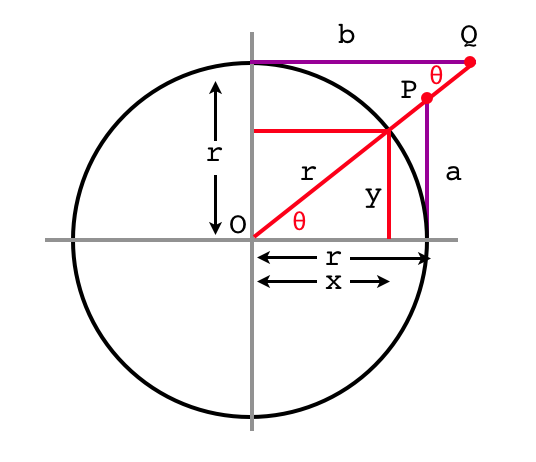
\includegraphics [scale=0.5] {sixfuncs1.png} \end{center}
\begin{center} 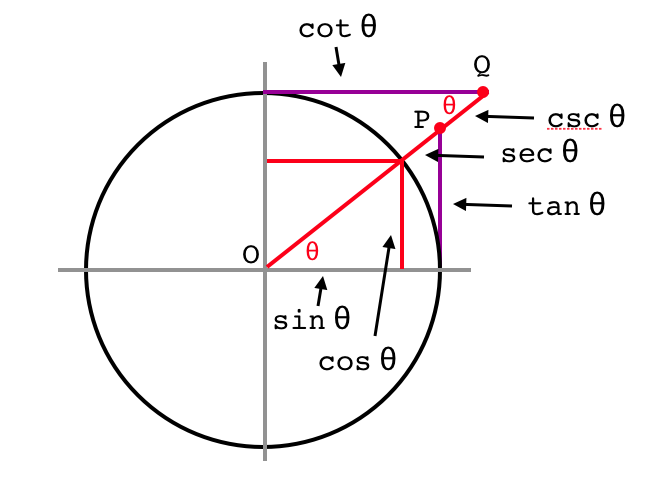
\includegraphics [scale=0.5] {sixfuncs2.png} \end{center}

Note:  the above diagram has an error, sine and cosine are switched.  I have to find the original figure (or redraw) to change this.
\end{document}  